% Options for packages loaded elsewhere
\PassOptionsToPackage{unicode}{hyperref}
\PassOptionsToPackage{hyphens}{url}
%
\documentclass[
  english,
  man]{apa6}
\usepackage{lmodern}
\usepackage{amssymb,amsmath}
\usepackage{ifxetex,ifluatex}
\ifnum 0\ifxetex 1\fi\ifluatex 1\fi=0 % if pdftex
  \usepackage[T1]{fontenc}
  \usepackage[utf8]{inputenc}
  \usepackage{textcomp} % provide euro and other symbols
\else % if luatex or xetex
  \usepackage{unicode-math}
  \defaultfontfeatures{Scale=MatchLowercase}
  \defaultfontfeatures[\rmfamily]{Ligatures=TeX,Scale=1}
\fi
% Use upquote if available, for straight quotes in verbatim environments
\IfFileExists{upquote.sty}{\usepackage{upquote}}{}
\IfFileExists{microtype.sty}{% use microtype if available
  \usepackage[]{microtype}
  \UseMicrotypeSet[protrusion]{basicmath} % disable protrusion for tt fonts
}{}
\makeatletter
\@ifundefined{KOMAClassName}{% if non-KOMA class
  \IfFileExists{parskip.sty}{%
    \usepackage{parskip}
  }{% else
    \setlength{\parindent}{0pt}
    \setlength{\parskip}{6pt plus 2pt minus 1pt}}
}{% if KOMA class
  \KOMAoptions{parskip=half}}
\makeatother
\usepackage{xcolor}
\IfFileExists{xurl.sty}{\usepackage{xurl}}{} % add URL line breaks if available
\IfFileExists{bookmark.sty}{\usepackage{bookmark}}{\usepackage{hyperref}}
\hypersetup{
  pdftitle={The subjective experience of O*NET work experiences as demands and resources},
  pdfauthor={Alicia Stachowski1, Renata Garcia Prieto Palacios Roji2, \& John Kulas2},
  pdflang={en-EN},
  pdfkeywords={keywords},
  hidelinks,
  pdfcreator={LaTeX via pandoc}}
\urlstyle{same} % disable monospaced font for URLs
\usepackage{graphicx,grffile}
\makeatletter
\def\maxwidth{\ifdim\Gin@nat@width>\linewidth\linewidth\else\Gin@nat@width\fi}
\def\maxheight{\ifdim\Gin@nat@height>\textheight\textheight\else\Gin@nat@height\fi}
\makeatother
% Scale images if necessary, so that they will not overflow the page
% margins by default, and it is still possible to overwrite the defaults
% using explicit options in \includegraphics[width, height, ...]{}
\setkeys{Gin}{width=\maxwidth,height=\maxheight,keepaspectratio}
% Set default figure placement to htbp
\makeatletter
\def\fps@figure{htbp}
\makeatother
\setlength{\emergencystretch}{3em} % prevent overfull lines
\providecommand{\tightlist}{%
  \setlength{\itemsep}{0pt}\setlength{\parskip}{0pt}}
\setcounter{secnumdepth}{-\maxdimen} % remove section numbering
% Make \paragraph and \subparagraph free-standing
\ifx\paragraph\undefined\else
  \let\oldparagraph\paragraph
  \renewcommand{\paragraph}[1]{\oldparagraph{#1}\mbox{}}
\fi
\ifx\subparagraph\undefined\else
  \let\oldsubparagraph\subparagraph
  \renewcommand{\subparagraph}[1]{\oldsubparagraph{#1}\mbox{}}
\fi
% Manuscript styling
\usepackage{upgreek}
\captionsetup{font=singlespacing,justification=justified}

% Table formatting
\usepackage{longtable}
\usepackage{lscape}
% \usepackage[counterclockwise]{rotating}   % Landscape page setup for large tables
\usepackage{multirow}		% Table styling
\usepackage{tabularx}		% Control Column width
\usepackage[flushleft]{threeparttable}	% Allows for three part tables with a specified notes section
\usepackage{threeparttablex}            % Lets threeparttable work with longtable

% Create new environments so endfloat can handle them
% \newenvironment{ltable}
%   {\begin{landscape}\begin{center}\begin{threeparttable}}
%   {\end{threeparttable}\end{center}\end{landscape}}
\newenvironment{lltable}{\begin{landscape}\begin{center}\begin{ThreePartTable}}{\end{ThreePartTable}\end{center}\end{landscape}}

% Enables adjusting longtable caption width to table width
% Solution found at http://golatex.de/longtable-mit-caption-so-breit-wie-die-tabelle-t15767.html
\makeatletter
\newcommand\LastLTentrywidth{1em}
\newlength\longtablewidth
\setlength{\longtablewidth}{1in}
\newcommand{\getlongtablewidth}{\begingroup \ifcsname LT@\roman{LT@tables}\endcsname \global\longtablewidth=0pt \renewcommand{\LT@entry}[2]{\global\advance\longtablewidth by ##2\relax\gdef\LastLTentrywidth{##2}}\@nameuse{LT@\roman{LT@tables}} \fi \endgroup}

% \setlength{\parindent}{0.5in}
% \setlength{\parskip}{0pt plus 0pt minus 0pt}

% \usepackage{etoolbox}
\makeatletter
\patchcmd{\HyOrg@maketitle}
  {\section{\normalfont\normalsize\abstractname}}
  {\section*{\normalfont\normalsize\abstractname}}
  {}{\typeout{Failed to patch abstract.}}
\patchcmd{\HyOrg@maketitle}
  {\section{\protect\normalfont{\@title}}}
  {\section*{\protect\normalfont{\@title}}}
  {}{\typeout{Failed to patch title.}}
\makeatother
\shorttitle{Title}
\keywords{keywords\newline\indent Word count: X}
\DeclareDelayedFloatFlavor{ThreePartTable}{table}
\DeclareDelayedFloatFlavor{lltable}{table}
\DeclareDelayedFloatFlavor*{longtable}{table}
\makeatletter
\renewcommand{\efloat@iwrite}[1]{\immediate\expandafter\protected@write\csname efloat@post#1\endcsname{}}
\makeatother
\usepackage{lineno}

\linenumbers
\usepackage{csquotes}
\ifxetex
  % Load polyglossia as late as possible: uses bidi with RTL langages (e.g. Hebrew, Arabic)
  \usepackage{polyglossia}
  \setmainlanguage[]{english}
\else
  \usepackage[shorthands=off,main=english]{babel}
\fi

\title{The subjective experience of O*NET work experiences as demands and resources}
\author{Alicia Stachowski\textsuperscript{1}, Renata Garcia Prieto Palacios Roji\textsuperscript{2}, \& John Kulas\textsuperscript{2}}
\date{}


\affiliation{\vspace{0.5cm}\textsuperscript{1} University of Wisconsin - Stout\\\textsuperscript{2} Montclair State University}

\abstract{
O*NET work characteristics were rated in terms of relevance, perception of demand, and perception as resource.
}



\begin{document}
\maketitle

The job demands-resources model (Demerouti, Bakker, Nachreiner, \& Schaufeli, 2001) and later job demands-resources theory (Bakker \& Demerouti, 2017) have inspired a plethora a study on the process and experience of job stress and employee motivation in recent decades. In the current project, we draw attention to a basic question regarding a key assumption we make regarding this process - that of the objective nature of job characteristics as either demands or resources. The major contribution of this project is to document whether job context and characteristics (pulled from O*NET) can simultaneously be classified as resources and as demands. We further present descriptive information regarding which job context and characteristics are rated the highest across jobs.

\hypertarget{the-job-demands-resources-theory}{%
\subsection{The Job demands-Resources Theory}\label{the-job-demands-resources-theory}}

The job demands-resources theory is an extension of the well-known job demands-resources model put forth by Demerouti and colleagues in 2001 (Demerouti et al., 2001). The job demands-resources model had been so heavily studied that a number of meta-analyses have been possible (e.g., (Crawford, LePine, \& Rich, 2010);
(Halbesleben, 2010); (Nahrgang, Morgeson, \& Hofmann, 2011)). The theory generated by the model integrates both the job design and job stress literatures to help explain the conditions under which a job would result in employee stress vs.~motivation (Bakker \& Demerouti, 2014). Per the job demands-resources theory, both work environment and job characteristics can be modeled via job demands and resources. Demerouti et al. (2001) define job demands broadly as components of a job that require sustained effort, and as such, produce psychological or physiological strain (e.g., high work pressure is frequently cited as a common demand). Resources, on the other hand, are physical, psychological, social, or organizational aspects of the job that may help an employee achieve work goals, reduce job demands, or promote personal growth and development (Demerouti et al., 2001).
Experiencing an element of one's job as a resource or demand activates one of two distinct processes: either health impairment (demands) or motivation (resources; (Bakker \& Demerouti, 2014). Job characteristics perceived to be demanding are effortful are frequently associated with negative outcomes such as exhaustion (e.g., Bakker, Demerouti, \& Schaufeli, 2003). On the other hand, job characteristics perceived as resources (fulfil psychological needs) are associated with positive organizational outcomes like engagement and motivation (Bakker, Hakanen, Demerouti, \& Xanthopoulou, 2007).

\hypertarget{objective-vs.-subjective-nature-of-demands-and-resources-the-role-of-appraisal}{%
\subsection{Objective vs.~Subjective Nature of Demands and Resources: The Role of Appraisal}\label{objective-vs.-subjective-nature-of-demands-and-resources-the-role-of-appraisal}}

Searle and Auton (2015) note that the majority of the research on workplace demands is based on apriori classifications of demands. However, the stress experience, or process, described early on by Lazarus and Folkman (1984) is grounded in the assumption that individual appraisals of stressors/demands vary. Their transactional theory or stress and coping states that people continuously appraise stimuli in their environments. An appraisal is the cognitive process whereby meaning is assigned to a stimulus. If a stimulus is appraised as a stressor (threat, challenge, potentially harmful), emotional distress leads to coping of some kind. This action to cope is also associated with another appraisal about the outcome itself and the process continues if the outcomes is not appraised as favorable (Lazarus \& Folkman, 1984). The stress appraisal process suggests that classifying a job characteristic or environmental condition as an objective demand or resource might be in error.
We next consider the (limited) empirical evidence on this topic. First, some relatively recent research suggests that job demands and resources may not be universally appraised or assigned as such. Starting with job demands, Webster, Beehr, and Love (2011), for example, studied workload, role ambiguity, and role conflict demands, and found while that each could be appraised primarily as challenges or hindrances demands, they could also simultaneously be perceived as being both a challenge and hinderance to different degrees. While their study did include resources, it nonetheless points to individual difference on how people perceive stressors at work. Although part of a much larger study on retirement, Sonnega, Helppie-McFall, Hudomiet, Willis, and Fisher (2018) compared self-reported (subjective) ratings of degree of physical demand, stress, and need for intense concentration from the Health and Retirement Study with objective ratings from O*Net. Correlations physical demand (r = .52), stress (r = .10), and need for intense concentration (r = .14), again suggesting perhaps that our objective ratings of job demands (and resources) may be subject to a greater level of individual difference than assumed. Next considering resources, Schmitz, McCluney, Sonnega, and Hicken (2019) captured subjective and objective resources in their study of retirement also. Correlations of composite variables for the resources of autonomy (r = .12), recognition of work (r = .07), decision freedom (r = .08), and advancement (r = -.01), while significant, certainly do not reflect high levels of overlap.
We do acknowledge as well, that demands and resources are not necessarily consistent across days, or seasons, for many employees. Downes, Reeves, McCormick, Boswell, and Butts (2021) meta-analysis addresses this reality in depth, although it is beyond the scope of this project.

\hypertarget{current-study-and-hypotheses}{%
\subsection{Current Study and Hypotheses}\label{current-study-and-hypotheses}}

The current study aims to explore the degree to which job context and job characteristic items from O*Net are considered demands and resources. Given theoretical and empirical findings, it seems quite plausible that our apriori assignment of job elements to a \enquote{demand} or \enquote{resource} category may be too simplistic. We aim to document a list of the highest rated demands and resources, as well as information on overlap of job characteristics as demands and resources, in addition to addressing the following predictions.

\hypertarget{current-study-and-research-questions-for-other-studies-notes}{%
\subsection{Current Study and Research Questions for other studies + notes}\label{current-study-and-research-questions-for-other-studies-notes}}

\hypertarget{study-2-introduction-correlates-with-engagement-and-stress}{%
\section{Study 2 Introduction: Correlates with Engagement and Stress}\label{study-2-introduction-correlates-with-engagement-and-stress}}

Research on the job demands-resources model (Demerouti et al., 2001) and later job demands-resources theory (Bakker \& Demerouti, 2017) highlight the importance of work characteristics on the experience of motivation and strain, which clearly have an impact on job performance. In this paper, we extend this critical research to that of the distinction between challenge and hinderance demands (and resource) in the workplace, and how they relate to two important organizational outcomes: engagement and stress. Prior to presenting the current study in detail, we provide a brief overview of the relevant theories and relevant empirical work on this topic.

\hypertarget{the-job-demands-resources-theory-1}{%
\subsection{The Job demands-Resources Theory}\label{the-job-demands-resources-theory-1}}

The overarching context for this study is that of the job demands-resources theory, which is an expansion of the well-studied job demands-resources model (Demerouti et al., 2001). One of the major advantages of the job demands-resources theory is that it allows us to model both work environment and job characteristics via job resources and demands. \emph{Resources} include physical, psychological, social, or organizational aspects of the job that may help an employee achieve work goals, reduce job demands, or promote personal growth and development (Demerouti et al., 2001). In contrast, demands include components of a job that require sustained effort, and as such, produce psychological or physiological strain (e.g., high work pressure is frequently cited as a common demand; Demerouti et al. (2001)).

Cognitively, the perception of an element of one's job as a resource or demand activates one of two distinct processes: either health impairment (resulting from demands) or motivation (resulting from resources) (Bakker \& Demerouti, 2014). Pertinent to the current study, demanding job characteristics are frequently often associated with negative outcomes (e.g., Bakker et al., 2003), whereas job characteristics deemed resources have been associated with positive organizational outcomes like engagement and motivation (Bakker et al., 2007).

\hypertarget{the-essential-role-of-appraisal}{%
\subsection{The Essential Role of Appraisal}\label{the-essential-role-of-appraisal}}

As implied in the last paragraph, job context and characteristics are \enquote{assigned} or appraised as demands or resources. Although some research on job demands in particular is based on apriori classifications of demands (Searle \& Auton, 2015), the classification of a work characteristic as a demand or resource is largely subjective by nature (e.g., an employee could most certainly perceive being a public figure as a resource or as a demand. The stress process speaks to how such individual difference in appraisal is possible. Lazarus and Folkman (1984) presented the transactional theory of stress and coping, which states that people cognitively appraise stimuli in their environments on a continuous basis. Via this process, meaning is assigned to stimuli -- if appraised as threatening, challenging, or possibly harmful, the resulting emotional distress initiates coping. The cycle of appraisal then continues based on the action to cope with the stressor (Lazarus \& Folkman, 1984).

\hypertarget{the-challenge-hinderance-framework}{%
\subsection{The Challenge-Hinderance Framework}\label{the-challenge-hinderance-framework}}

Although there is a tendency to attach a negative connotation to the word \enquote{stress}, Selye (1936) defined stress as a response to change, which is quite non-specific. We return to the employed public figure for this next section. It is quite probable that two employees would be called upon to serve as a spokesperson for their organization in a time of need. One may appraise the circumstance as an opportunity to positively influence others, while the other may plausibly feel paralyzed by the task. Cavanaugh, Boswell, Roehling, and Boudreau (2000) delineated between two forms of demands -- that of \emph{challenge} and \emph{hinderance} demands. Challenge demands promote mastery, personal growth, and future gains. Hinderance demands, in contrast, inhibit growth, learning and goal achievement. This particular distinction has been of value in determining what demands are related to various outcomes, whereby challenge stressors are typically associated with positive outcomes, and hinderance stressors, negative outcomes (e.g., Cavanaugh et al. (2000)). However, one of the key questions we need to ask as researchers pertains to the very basic consideration of appraisals.

We next consider the empirical evidence on this topic. The first obvious question is whether people perceive demands as challenges vs.~hinderances, or whether all demands are under a larger \enquote{demands} category. Evidence suggests the employees do, in fact, distinguish between challenge and hinderance stressors (e.g., Bakker \& Sanz-Vergel, 2013; Gerich, 2017; Webster et al., 2011). For example, Bakker and Sanz-Vergel (2013) found that perceived work pressure as a hinderance demand, and emotional demands as more of a challenge demand. Webster et al. (2011) approached this question with three common workplace demands: workload, role ambiguity, and role conflict. They found while that each could be appraised primarily as challenges or hindrances demands, they could also simultaneously be perceived as being both a challenge and hinderance to different degrees.
While their study did include resources, it nonetheless points to the possibility that demands might be differentially appraised and related to outcomes (e.g., Podsakoff, LePine, \& LePine, 2007). The challenge-hinderance framework has, in fact, been associated with a wide variety of organizational outcomes ranging from affective variables like job satisfaction, to motivation, performance, and well-being. A sampling of variables and relationships are described below to provide a sense of scope of the work that has been on this topic. For example, Cavanaugh et al. (2000), in a study of managers, found that challenge demands were positively related to job satisfaction and negatively related to job search behaviors, while hinderance demands demonstrated the opposite pattern. In contrast, Abbas and Raja (2019) found that challenge and hindrance stressors were \emph{both} positively related to strain and turnover intensions. We also have some evidence that challenge-hinderance appraisals are related to engagement in the expected direction whereby hinderance appraisals are negatively associated with engagement and challenge appraisals are positively associated with it (Crawford et al., 2010). Challenge and hinderance appraisals have also been shown to relate to citizenship and counterproductive performance, although indirectly via emotions like anxiety (Rodell \& Judge, 2009). Lastly, Gerich (2017) concluded that employee well-being was also, in part, explained by appraised challenge or hinderance demands such that working conditions of time pressure, qualitative demands, responsibility, and interruptions, were partially mediated by challenge and hinderance demands.
We even have sufficient evidence to explore outcomes associated with challenge and hinderance stressors meta-analytically at this point. Podsakoff et al. (2007) supported the original assertion of Cavanaugh et al. (2000) with regard to work outcomes such that challenge stressors were positively related to job satisfaction and organizational commitment, and negatively related to both turnover intentions and actual turnover. The opposite pattern of relationship was observed for hinderance stressors.

\hypertarget{current-study-and-hypotheses-1}{%
\subsection{Current Study and Hypotheses}\label{current-study-and-hypotheses-1}}

Given the abundance of theoretical and empirical support for the connection between resources and positive organizational outcomes, and between demands and negative resources, we sought to explore whether or not the appraisal of a demand as a challenge or hinderance would be related \emph{differently} to two organizational outcomes: engagement (a positive affective experience defined as a fulfilling, work-related state of mind characterized by vigor, dedication, and absorption, schaufeli2002measurement{]}, workplace stress (``an individual state characterized by a combination of high arousal and displeasure'', p.~15, Pejtersen, Kristensen, Borg, \& Bjorner, 2010) and burnout {[}\enquote{`The degree of physical and psychological fatigue and exhaustion that is perceived by the person as related to his/her work}, p.~197; Kristensen, Borritz, Villadsen, and Christensen (2005);negative affective experiences). Drawing on the job demands-resources theory and the challenge-hinderance framework, we propose that job elements appraised as \enquote{challenge demands} (i.e., promote mastery, personal growth, and future gains) would activate (be related to) a positive state -- that of engagement. In contrast, elements of one's job appraised as a hinderance demand (i.e., inhibit growth, learning and goal achievement) would activate a negative state -- here, stress.

These are extra sources below if we want more information. The intro is getting a little bit long for this one.
Edwards, Franco-Watkins, Cullen, Howell, and Acuff Jr (2014) (this one is interesting -- manipulated challenge and hinderance stress by offering money/taking it away based on the correctness of their decisions - of university students and measured outcomes\ldots{} potentially include this in the discussion section i)
Kim and Beehr (2018)
Searle and Auton (2015)
Tuckey et al. (2015)
Webster, Beehr, and Christiansen (2010)

\hypertarget{methods}{%
\section{Methods}\label{methods}}

Bakker and Demerouti (2017) claim that their JD-R model has been used by, \enquote{\ldots many Occupational Health and Safety/Workplace Health \& Safety regulators and government agencies around the world} (p.~273). The current study expands upon this integration by considering the crosswalk between the JD-R and O*Net.

\hypertarget{study-1}{%
\subsection{Study 1}\label{study-1}}

Bakker and Demerouti (2017) state that, \enquote{\ldots research has shown that challenge demands may be experienced as hindrance demands (and vice versa) depending on the context} (p.~278). We extend this acknowlegement by investigating whether some characteristics of work may also vacillate between demand and \emph{resource}.

\begin{quote}
\emph{Hypothesis 1}: Job characteristics differ in variability/stability regarding subjective worker perception as a demand or resource.
\end{quote}

\begin{quote}
\emph{Hypothesis 2}: Job characteristics with the greatest variability will have industrial moderators.
\end{quote}

\hypertarget{participants}{%
\subsection{Participants}\label{participants}}

Of the 785 Prolific panel individuals who initially accessed the survey link, 112 indicated that they were not interested, had more than 200 missing responses, or had 20 or more identical consecutive sequential responses (Yentes \& Wilhelm, 2021). Applying a further screen regarding attention checks (there were four attention checks embedded throughout, asking respondents to indicate a specific answer) resulted in the retention of 568 respondents who constitute the current SIOP sample. 13.57\% had been in their referent job less than 6 months, 19.20\% between 6 months and a year, 49.12\% between one and five years, 13.27\% between 5 and 10 years, and 4.87\% more than 10 years.

Ages ranged from 18 to 65 with an average of 28.18 years old (SD = 7.53). The survey offered a free-field gender identity category, although the sample predominantly self-identified as female (52.58\%) or male (46.83\%). Jobs were classified into the International Standard Classification of Occupations (ISCO) via the package labourR (Kouretsis, Bampouris, Morfiris, \& Papageorgiou, 2020). We further grossly categorized these classifications into \enquote{knowledge} (\emph{n} = 320) versus \enquote{service} (\emph{n} = 214) occupations with knowledge workers being ISCO classifications of: 1) Professionals, and 2) Managers.

\hypertarget{top-10-demands-and-resources-divided-by-skilled-versus-knowledge-workers}{%
\subsection{top 10 demands and resources, divided by skilled versus knowledge workers}\label{top-10-demands-and-resources-divided-by-skilled-versus-knowledge-workers}}

\hypertarget{resources---top-10}{%
\subsection{Resources - Top 10}\label{resources---top-10}}

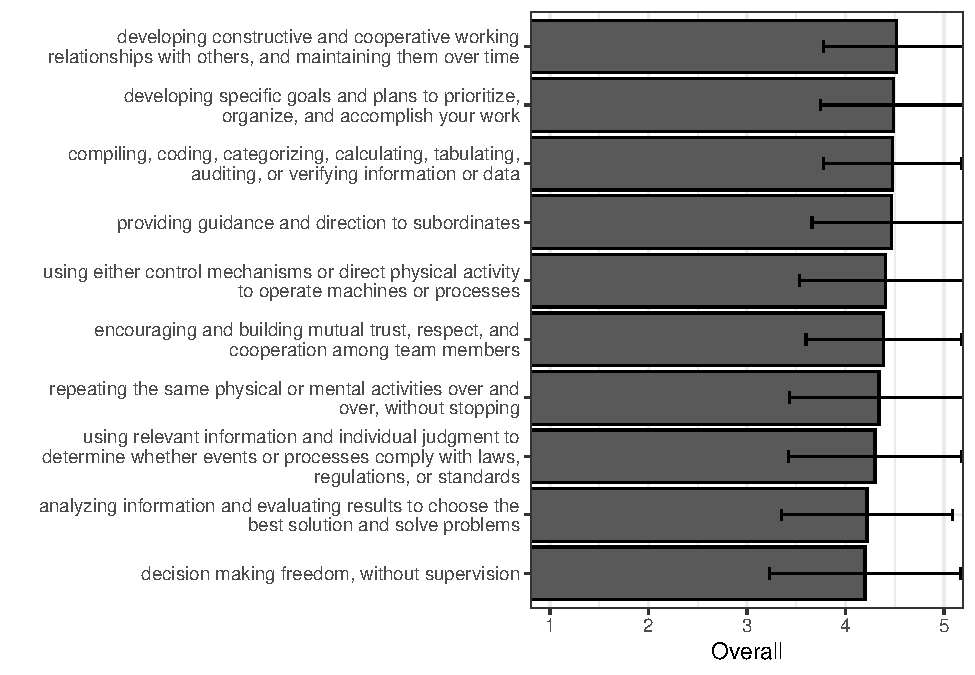
\includegraphics{SIOPjdr2_files/figure-latex/unnamed-chunk-1-1.pdf}

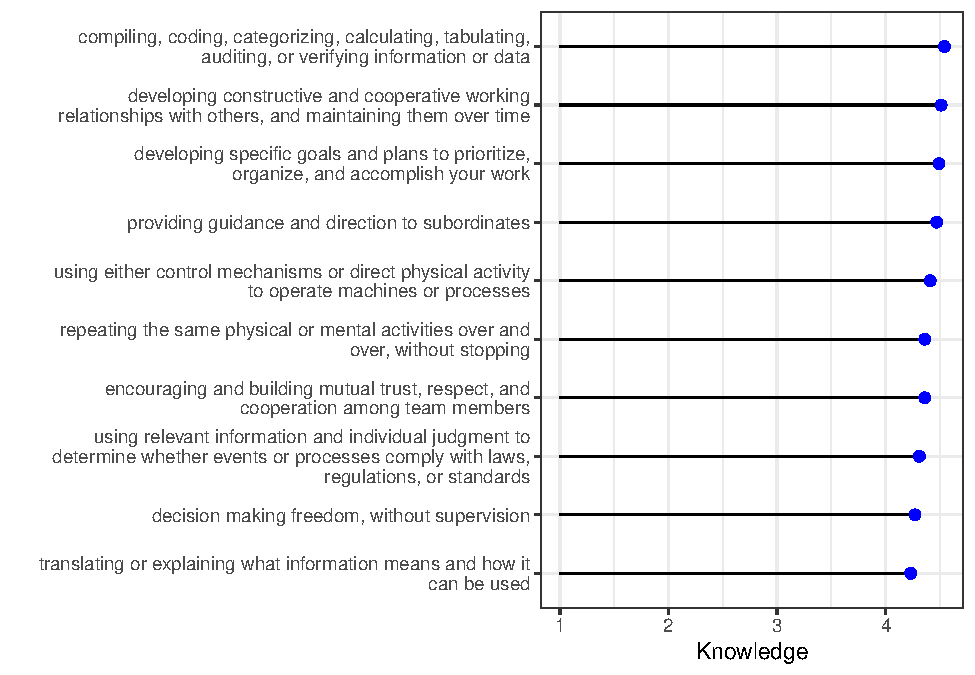
\includegraphics{SIOPjdr2_files/figure-latex/unnamed-chunk-2-1.pdf}

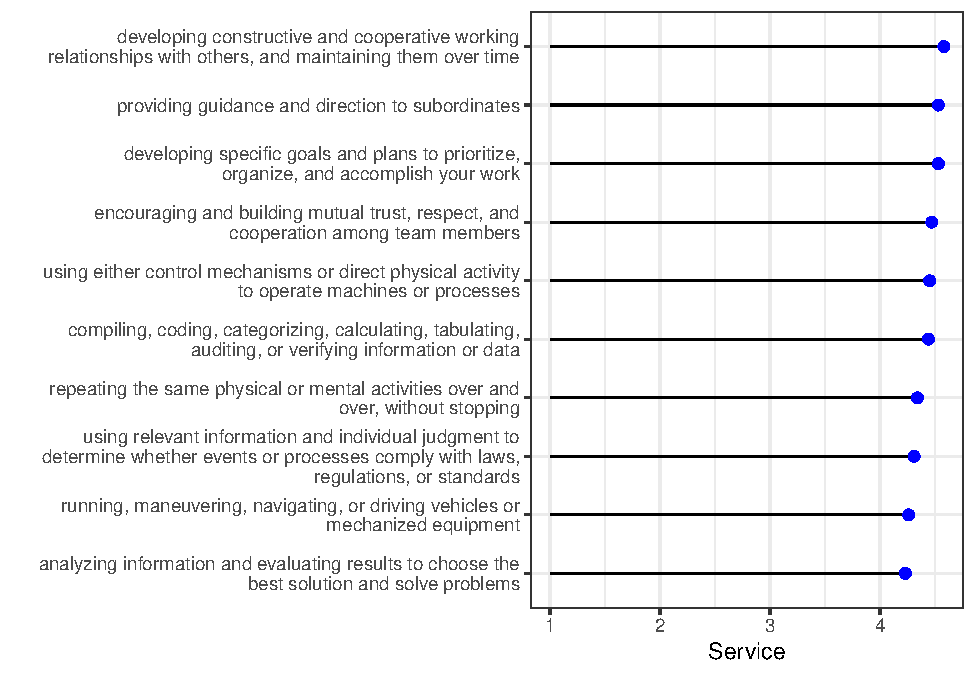
\includegraphics{SIOPjdr2_files/figure-latex/unnamed-chunk-3-1.pdf}

\hypertarget{challenge-demands---top-10}{%
\subsection{Challenge Demands - Top 10}\label{challenge-demands---top-10}}

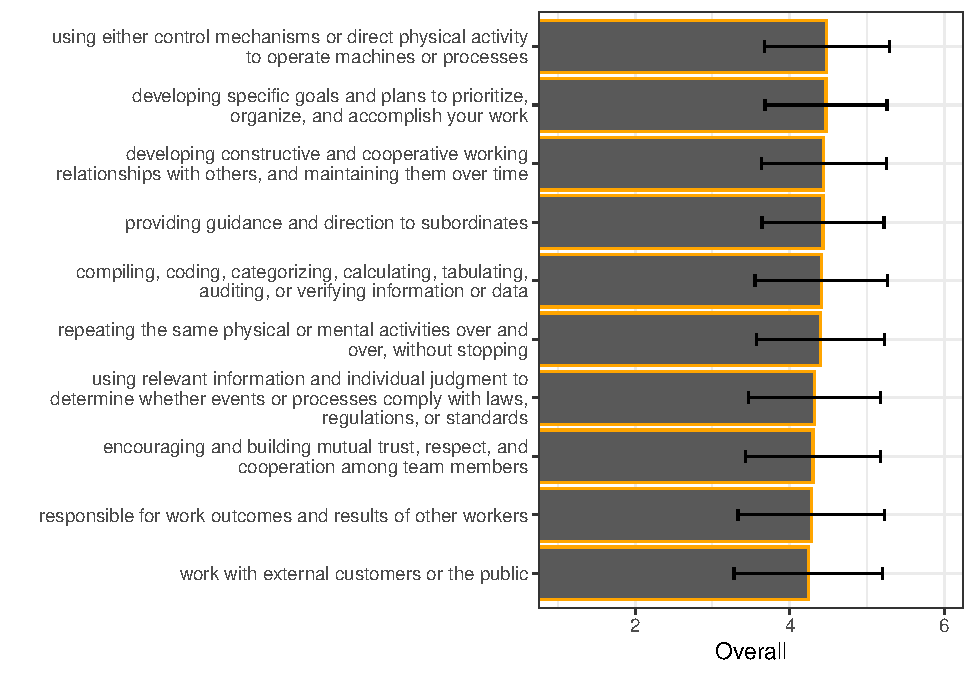
\includegraphics{SIOPjdr2_files/figure-latex/unnamed-chunk-4-1.pdf}

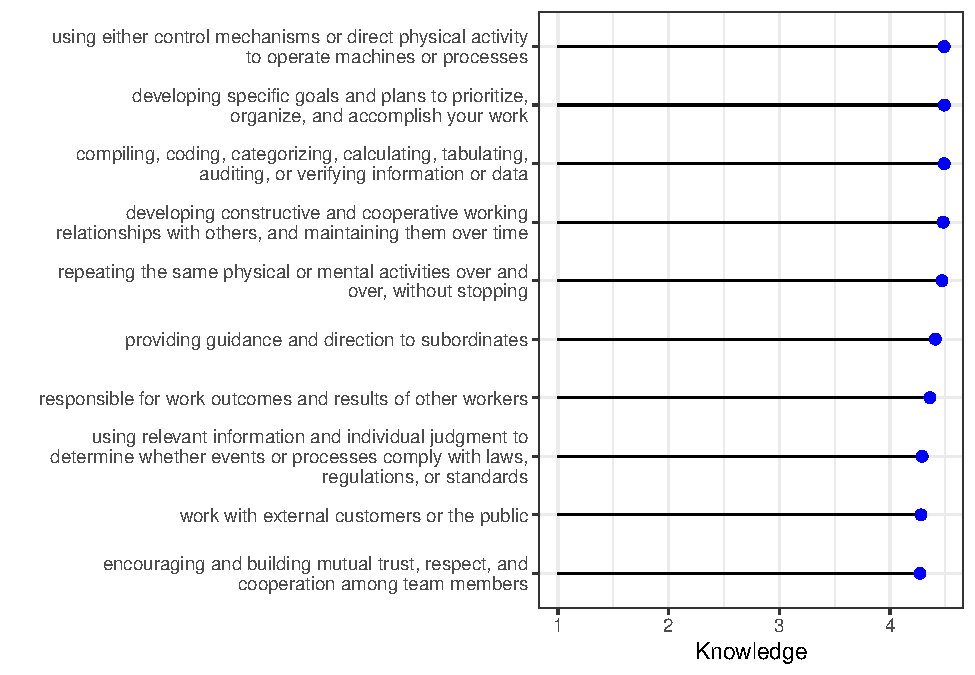
\includegraphics{SIOPjdr2_files/figure-latex/unnamed-chunk-5-1.pdf}

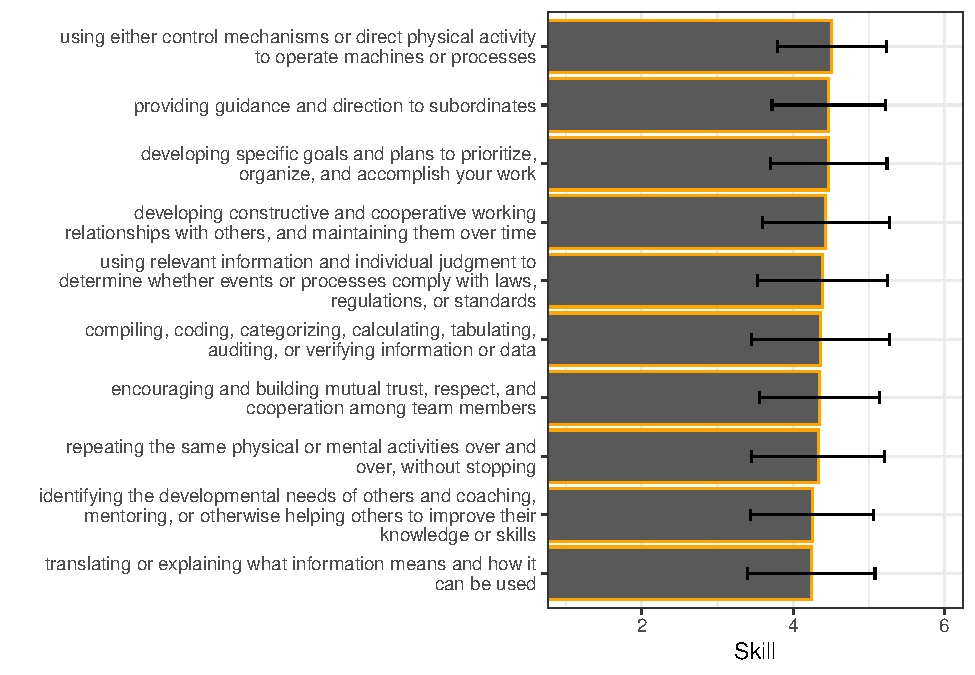
\includegraphics{SIOPjdr2_files/figure-latex/unnamed-chunk-6-1.pdf}
\#\# Hindrance Demands - Top 10

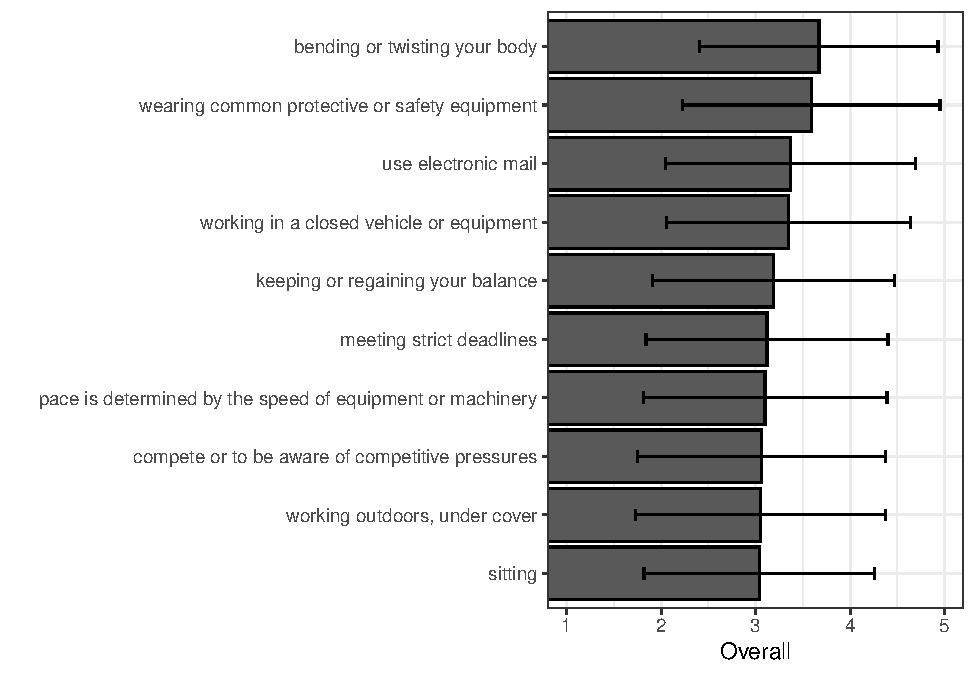
\includegraphics{SIOPjdr2_files/figure-latex/unnamed-chunk-7-1.pdf}

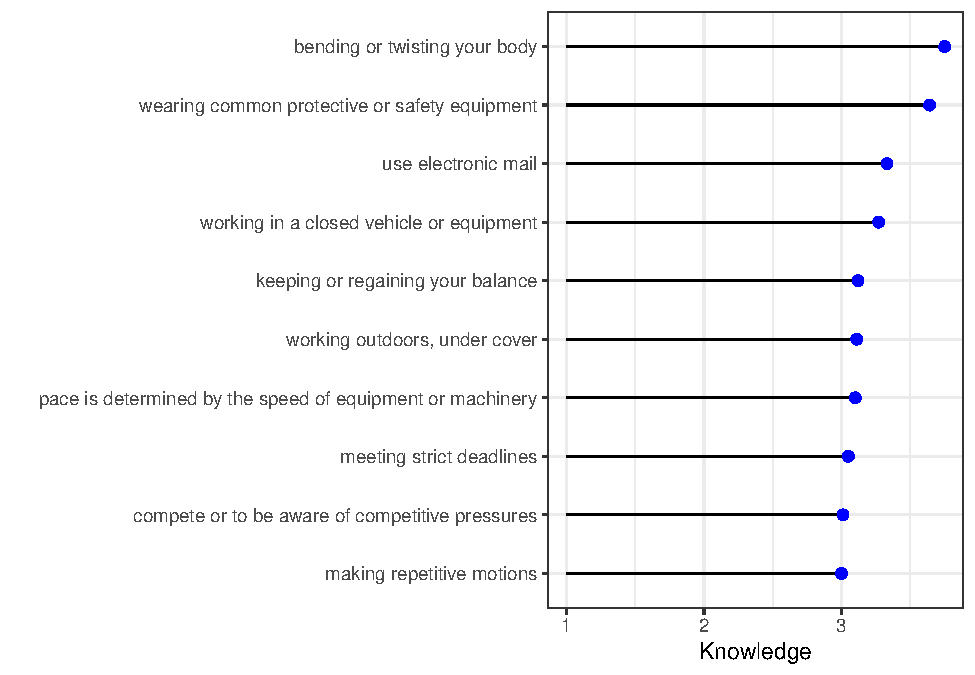
\includegraphics{SIOPjdr2_files/figure-latex/unnamed-chunk-8-1.pdf}

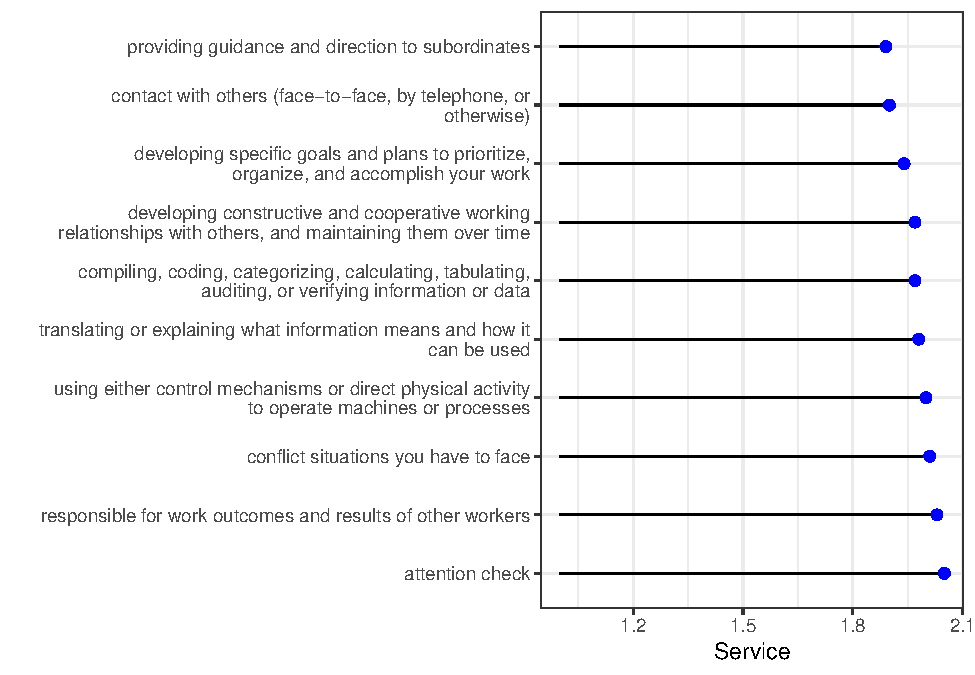
\includegraphics{SIOPjdr2_files/figure-latex/unnamed-chunk-9-1.pdf}

\hypertarget{hypothesis-2}{%
\subsubsection{Hypothesis 2}\label{hypothesis-2}}

Hypothesis 2a predicted that job demands with the greatest variability would be moderated by worker type.

Hypothesis 2b predicted that job resources with the greatest variability would be moderated by worker type.

The top 10 resources with the most variability in ratings yeilded standard deviations of 0.64 to 0.93. T-tests for each of these were conducted and are presented in table XX.

The top 10 hindrance demands with the most variability in ratings yeilded standard deviations of 1.17 to 1.38. T-tests for each of these were conducted and are presented in table XX.

The top 10 challenge demands with the most variability in ratings yeilded standard deviations of 0.77 to 0.95. T-tests for each of these were conducted and are presented in table XX.

\hypertarget{low-variability-demands-and-resources}{%
\section{Low Variability Demands and Resources}\label{low-variability-demands-and-resources}}

The below graphs present the resources, challenges, and hindrances that are \emph{largely agreed on} as indexed by low standard deviations

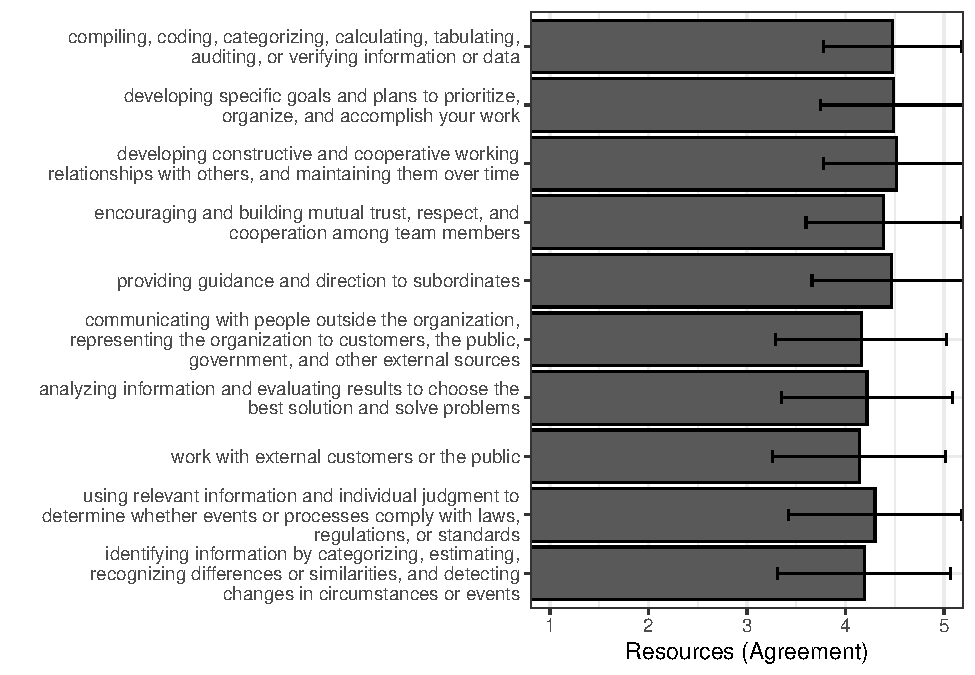
\includegraphics{SIOPjdr2_files/figure-latex/resourceslowsd-1.pdf}

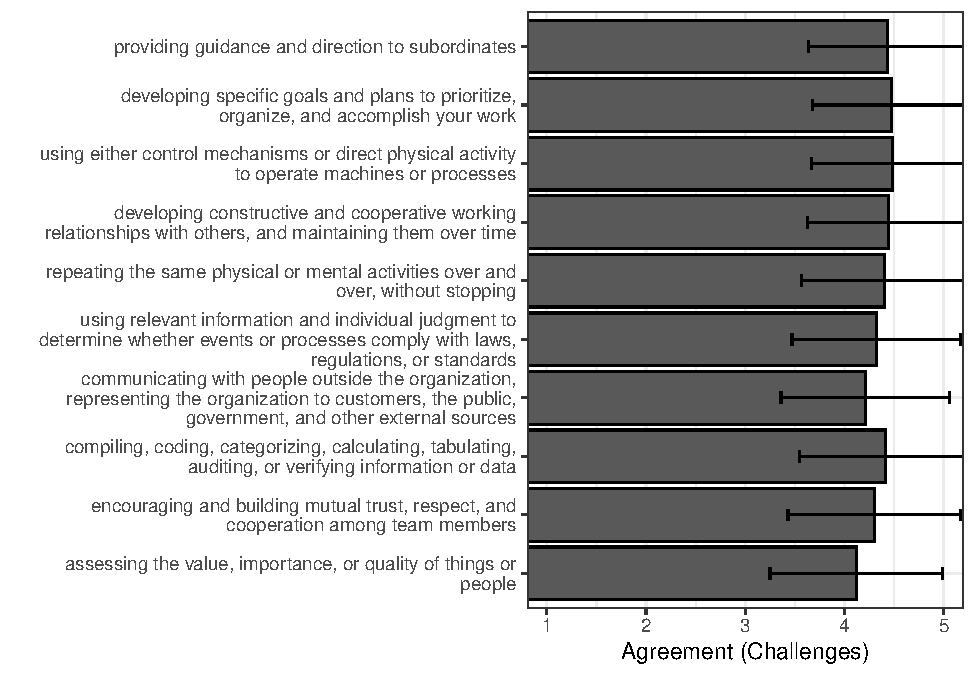
\includegraphics{SIOPjdr2_files/figure-latex/challengesagree-1.pdf}

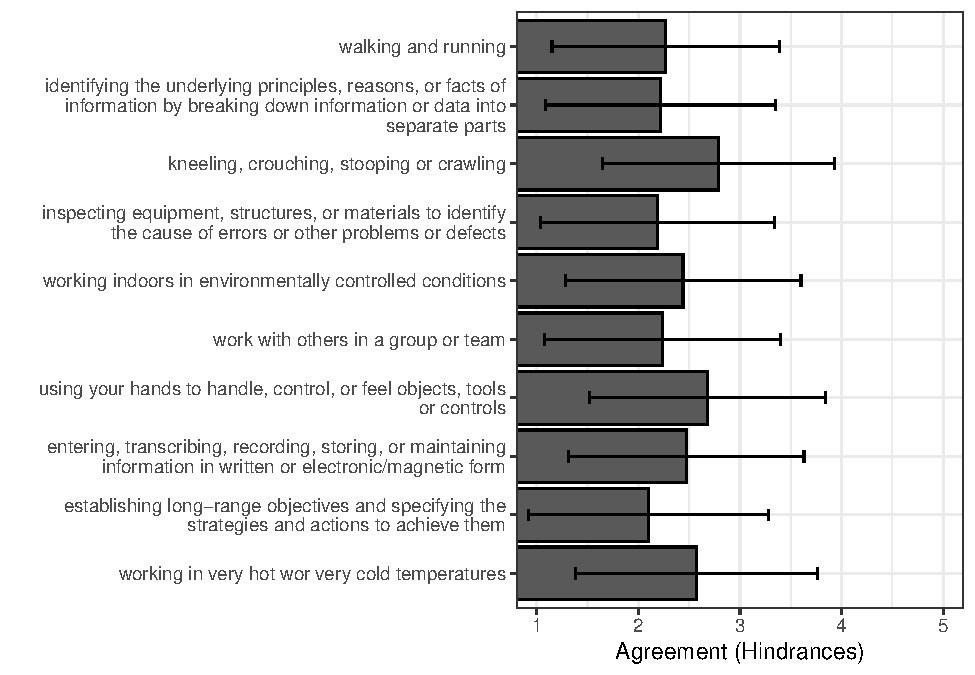
\includegraphics{SIOPjdr2_files/figure-latex/hindrancesagree-1.pdf}

As can be seen by the graphs, there is considerable disagreement regarding the degree to which job elements are considered \emph{hindrances}, with the 10 elements showing the greatest agreement still ranging in standard deviations from 1.12 to 1.19. What is widely seen as a resource and challenge tends to be more universally agreed upon (range of lowest 10 resource standard deviations is 0.70 to 0.88 and the range of lowest 10 challenge standard deviations is 0.79 to 0.87.

\hypertarget{study-3}{%
\subsection{Study 3}\label{study-3}}

In an attempt to integrate the O*NET taxonomy within the orientation of the Job Demands-Resources (Bakker \& Demerouti, 2017; Bakker et al., 2003; Demerouti et al., 2001), a series of evaluations were made that used: 1) O*NET terminology (both descriptor and response option), 2) JD-R influenced ratings of demand, challenge, or hindrance. The outcome of this integration is a cross-walk between the Department of Labor classifications and the I-O literature steeped JD-R. While O*Net provides thorough documentation of information associated with job analyses, one of the remaining limitations is its lack of connection to theory. Given the popularity of the Job Demands-Resources Theory (JD-R; Demerouti et al., 2001) in exploring questions related to everything from motivation to job design, we aim to explore the intersection between perceptions of job demands and resources, and the broad set of job characteristics provided on O*Net. In an attempt to integrate the O*Net taxonomy within the orientation of the JD-R framework (Bakker \& Demerouti, 2017; Bakker et al., 2003; Demerouti et al., 2001), a series of evaluations were made that used: 1) direct O*Net terminology (both descriptor and response option), and 2) JD-R influenced ratings of demand, challenge, or hindrance. Prior to a description of results, a brief overview of both the JD-R theory and O*Net is provided.

\#\#The Job demands-Resources Theory

The overarching context for this study is that of the job demands-resources theory, which is an expansion of the well-studied job demands-resources model (Demerouti et al., 2001). One of the major advantages of the job demands-resources theory is that it allows us to model both work environment and job characteristics via job resources and demands. \emph{Resources} include physical, psychological, social, or organizational aspects of the job that may help an employee achieve work goals, reduce job demands, or promote personal growth and development (Demerouti et al., 2001). In contrast, demands include components of a job that require sustained effort, and as such, produce psychological or physiological strain (e.g., high work pressure is frequently cited as a common demand; Demerouti et al. (2001)).
Cognitively, the perception of an element of one's job as a resource or demand activates one of two distinct processes: either health impairment (resulting from demands) or motivation (resulting from resources) (Bakker \& Demerouti, 2014). Pertinent to the current study, demanding job characteristics are frequently often associated with negative outcomes (e.g., {\textbf{???}}), whereas job characteristics deemed resources have been associated with positive organizational outcomes like engagement and motivation ({\textbf{???}}).

\hypertarget{onet-resource}{%
\subsection{O*Net Resource}\label{onet-resource}}

Originally, the Advisory Panel for the Dictionary of Occupational Titles recommended a system that would \enquote{\ldots promote the effective education, training, counseling, and employment of the American workforce. It should accomplish its purpose by providing a database system that identified, defines, classifies, and describes occupations in the economy in an accessible and flexible manner} (Dictionary of Occupational Titles (US) and Service (1993), p.~6). The result was the now commonly used O*NET. The Occupational Information Network (O*NET; onetonline.org) contains a comprehensive description of occupations (Peterson et al., 2001). This widely accessed database houses hundreds of standardized and occupation-specific descriptors most occupations in the US and these descriptions are continually updated. In fact, there was a call to work with experienced I/O psychologists over the summer to update the content for the Industrial and Organizational Psychologist listing on O*Net (\url{https://www.onetonline.org/link/summary/19-3032.00}). These data, and the tools provided for free on the website (e.g., Career Exploration Tools, \enquote{My Next Move for Veterans}, \enquote{My Next Move}, Toolkit for Business) are frequently used by counselors, students, human resources departments, and researchers to assist potential applicants discover the skills and training they need for the job of their choice, and also employers with information with which to craft job descriptions and help employees determine what skills are needed for promotion.

\hypertarget{current-study}{%
\subsection{Current Study}\label{current-study}}

Interestingly, we have not yet integrated this practical and accessible resource within the JD-R framework. This paper aims to provide such a crosswalk or integration of the theory and practical occupations-focused data on O*Net. Several broad research questions are examined across jobs:
\textgreater{}\emph{Research Question 1}: Which O*Net job characteristics are consistently rated as job resources?
\textgreater{}\emph{Research Question 2}: Which O*Net job characteristics are consistently rated as challenge demands?
\textgreater{}\emph{Research Question 3}: Which O*Net job characteristics are consistently rated as hinderance demands?

The other distinct possibility we expect we may observe is wide variability in the assignment of some job characteristics within the JD-R framework. In fact, a growing body of evidence suggests people may not universally experience job characteristics as challenges or hinderances (e.g., (Bakker \& Sanz-Vergel, 2013); {[}cavanaugh2000empirical{]}; (Gerich, 2017); (Podsakoff et al., 2007); (Webster et al., 2011)). Thus, a fourth question of interest explores just that possibility.
Research Question 4: Which O*Net job characteristics show wide variability in assigned JD-R classification of resource, challenge, or hinderance.

\hypertarget{results}{%
\section{Results}\label{results}}

Average rating of each category by item and focus on the ones with low SDs.

\hypertarget{discussion}{%
\section{Discussion}\label{discussion}}

Could be another piece of info onet uses along with descriptions -- could list resource challenge hinderance

\hypertarget{materials}{%
\subsection{Materials}\label{materials}}

\hypertarget{characteristics-demands-and-resources}{%
\subsubsection{Characteristics, Demands, and Resources}\label{characteristics-demands-and-resources}}

We used 98 statements taken from O*NET \href{https://www.O*NETonline.org/find/descriptor/result/4.A.1.b.3}{\enquote{activity} and \enquote{context} classifications}. We retained 41 \enquote{work activity} classifications which O*NET groups into categories of \enquote{Information Input} (5 statements), \enquote{Interacting with Others} (17 statements), \enquote{Mental Processes} (10 statements) and \enquote{Work Output} (9 statements). 57 \enquote{work context} statements grouped into \enquote{Interpersonal Relationships} (14 statements), \enquote{Physical Work Conditions} (30 statements), and \enquote{Structural Job Characteristics} (13 statements).

These \enquote{desriptors} have response categories \href{https://www.O*NETonline.org/find/descriptor/result/4.C.1.c.2}{see for example}. We used the O*NET wording to capture characteristics of relevance for each respondent. Subsequent to these self evaluations, each respondent who agreed that the element had \emph{at least some relevance} to their job was also asked to rate that element in terms of, 1) \ldots this aspect of your job is a resource that can be functional in achieving work goals, reduce job demands, or stimulate personal growth/development, 2) \ldots this aspect of your job is a challenge that can promote mastery, personal growth, or future gains, and 3) \ldots this aspect of your job is a hinderance that can inhibit personal growth, learning, and work goal attainment.

Our intent was to use O*NET

\hypertarget{burnout-and-stress}{%
\subsubsection{Burnout and Stress}\label{burnout-and-stress}}

Were taken from the Copenhagen Psychosocial Questionnaire (Burr et al., 2019). There were 4 burnout items and 3 stress items.

Engagement
Demographics

\hypertarget{procedure}{%
\subsection{Procedure}\label{procedure}}

Qualtrics panel

\hypertarget{data-analysis}{%
\subsection{Data analysis}\label{data-analysis}}

We used R (Version 4.0.3; R Core Team, 2020) and the R-packages \emph{careless} (Version 1.1.3; Yentes \& Wilhelm, 2021), \emph{labourR} (Version 1.0.0; Kouretsis et al., 2020), \emph{papaja} (Version 0.1.0.9997; Aust \& Barth, 2020), and \emph{tinylabels} (Barth, 2021) for all our analyses.

\hypertarget{results-1}{%
\section{Results}\label{results-1}}

\hypertarget{discussion-1}{%
\section{Discussion}\label{discussion-1}}

\newpage

\hypertarget{references}{%
\section{References}\label{references}}

\begingroup
\setlength{\parindent}{-0.5in}
\setlength{\leftskip}{0.5in}

\hypertarget{refs}{}
\leavevmode\hypertarget{ref-abbas2019challenge}{}%
Abbas, M., \& Raja, U. (2019). Challenge-hindrance stressors and job outcomes: The moderating role of conscientiousness. \emph{Journal of Business and Psychology}, \emph{34}(2), 189--201.

\leavevmode\hypertarget{ref-R-papaja}{}%
Aust, F., \& Barth, M. (2020). \emph{papaja: Create APA manuscripts with R Markdown}. Retrieved from \url{https://github.com/crsh/papaja}

\leavevmode\hypertarget{ref-bakker2014job}{}%
Bakker, A. B., \& Demerouti, E. (2014). Job demands--resources theory. \emph{Wellbeing: A Complete Reference Guide}, 1--28.

\leavevmode\hypertarget{ref-bakker2017job}{}%
Bakker, A. B., \& Demerouti, E. (2017). Job demands--resources theory: Taking stock and looking forward. \emph{Journal of Occupational Health Psychology}, \emph{22}(3), 273.

\leavevmode\hypertarget{ref-bakker2007job}{}%
Bakker, A. B., Hakanen, J. J., Demerouti, E., \& Xanthopoulou, D. (2007). Job resources boost work engagement, particularly when job demands are high. \emph{Journal of Educational Psychology}, \emph{99}(2), 274.

\leavevmode\hypertarget{ref-bakker2013weekly}{}%
Bakker, A. B., \& Sanz-Vergel, A. I. (2013). Weekly work engagement and flourishing: The role of hindrance and challenge job demands. \emph{Journal of Vocational Behavior}, \emph{83}(3), 397--409.

\leavevmode\hypertarget{ref-bakker2003dual}{}%
Bakker, A., Demerouti, E., \& Schaufeli, W. (2003). Dual processes at work in a call centre: An application of the job demands--resources model. \emph{European Journal of Work and Organizational Psychology}, \emph{12}(4), 393--417.

\leavevmode\hypertarget{ref-R-tinylabels}{}%
Barth, M. (2021). \emph{tinylabels: Lightweight variable labels}. Retrieved from \url{https://github.com/mariusbarth/tinylabels}

\leavevmode\hypertarget{ref-burr_third_2019}{}%
Burr, H., Berthelsen, H., Moncada, S., Nübling, M., Dupret, E., Demiral, Y., \ldots{} Pohrt, A. (2019). The Third Version of the Copenhagen Psychosocial Questionnaire. \emph{Safety and Health at Work}, \emph{10}(4), 482--503. \url{https://doi.org/10.1016/j.shaw.2019.10.002}

\leavevmode\hypertarget{ref-cavanaugh2000empirical}{}%
Cavanaugh, M. A., Boswell, W. R., Roehling, M. V., \& Boudreau, J. W. (2000). An empirical examination of self-reported work stress among us managers. \emph{Journal of Applied Psychology}, \emph{85}(1), 65.

\leavevmode\hypertarget{ref-crawford2010linking}{}%
Crawford, E. R., LePine, J. A., \& Rich, B. L. (2010). Linking job demands and resources to employee engagement and burnout: A theoretical extension and meta-analytic test. \emph{Journal of Applied Psychology}, \emph{95}(5), 834.

\leavevmode\hypertarget{ref-demerouti2001job}{}%
Demerouti, E., Bakker, A. B., Nachreiner, F., \& Schaufeli, W. B. (2001). The job demands-resources model of burnout. \emph{Journal of Applied Psychology}, \emph{86}(3), 499.

\leavevmode\hypertarget{ref-advisory1993new}{}%
Dictionary of Occupational Titles (US), A. P. for the, \& Service, U. S. E. (1993). \emph{The new dot: A database of occupational titles for the twenty-first century}. US Department of Labor, Employment; Training Administration, US~\ldots.

\leavevmode\hypertarget{ref-downes2021incorporating}{}%
Downes, P. E., Reeves, C. J., McCormick, B. W., Boswell, W. R., \& Butts, M. M. (2021). Incorporating job demand variability into job demands theory: A meta-analysis. \emph{Journal of Management}, \emph{47}(6), 1630--1656.

\leavevmode\hypertarget{ref-edwards2014unifying}{}%
Edwards, B. D., Franco-Watkins, A. M., Cullen, K. L., Howell, J. W., \& Acuff Jr, R. E. (2014). Unifying the challenge-hindrance and sociocognitive models of stress. \emph{International Journal of Stress Management}, \emph{21}(2), 162.

\leavevmode\hypertarget{ref-gerich2017relevance}{}%
Gerich, J. (2017). The relevance of challenge and hindrance appraisals of working conditions for employees' health. \emph{International Journal of Stress Management}, \emph{24}(3), 270.

\leavevmode\hypertarget{ref-halbesleben2010meta}{}%
Halbesleben, J. R. (2010). A meta-analysis of work engagement: Relationships with burnout, demands, resources, and consequences. \emph{Work Engagement: A Handbook of Essential Theory and Research}, \emph{8}(1), 102--117.

\leavevmode\hypertarget{ref-kim2018challenge}{}%
Kim, M., \& Beehr, T. A. (2018). Challenge and hindrance demands lead to employees' health and behaviours through intrinsic motivation. \emph{Stress and Health}, \emph{34}(3), 367--378.

\leavevmode\hypertarget{ref-R-labourR}{}%
Kouretsis, A., Bampouris, A., Morfiris, P., \& Papageorgiou, K. (2020). \emph{LabourR: Classify multilingual labour market free-text to standardized hierarchical occupations}. Retrieved from \url{https://CRAN.R-project.org/package=labourR}

\leavevmode\hypertarget{ref-kristensen2005copenhagen}{}%
Kristensen, T. S., Borritz, M., Villadsen, E., \& Christensen, K. B. (2005). The copenhagen burnout inventory: A new tool for the assessment of burnout. \emph{Work \& Stress}, \emph{19}(3), 192--207.

\leavevmode\hypertarget{ref-lazarus1984stress}{}%
Lazarus, R. S., \& Folkman, S. (1984). \emph{Stress, appraisal, and coping}. Springer publishing company.

\leavevmode\hypertarget{ref-nahrgang2011safety}{}%
Nahrgang, J. D., Morgeson, F. P., \& Hofmann, D. A. (2011). Safety at work: A meta-analytic investigation of the link between job demands, job resources, burnout, engagement, and safety outcomes. \emph{Journal of Applied Psychology}, \emph{96}(1), 71.

\leavevmode\hypertarget{ref-pejtersen2010second}{}%
Pejtersen, J. H., Kristensen, T. S., Borg, V., \& Bjorner, J. B. (2010). The second version of the copenhagen psychosocial questionnaire. \emph{Scandinavian Journal of Public Health}, \emph{38}(3\_suppl), 8--24.

\leavevmode\hypertarget{ref-peterson2001understanding}{}%
Peterson, N. G., Mumford, M. D., Borman, W. C., Jeanneret, P. R., Fleishman, E. A., Levin, K. Y., \ldots{} others. (2001). Understanding work using the occupational information network (o* net): Implications for practice and research. \emph{Personnel Psychology}, \emph{54}(2), 451--492.

\leavevmode\hypertarget{ref-podsakoff2007differential}{}%
Podsakoff, N. P., LePine, J. A., \& LePine, M. A. (2007). Differential challenge stressor-hindrance stressor relationships with job attitudes, turnover intentions, turnover, and withdrawal behavior: A meta-analysis. \emph{Journal of Applied Psychology}, \emph{92}(2), 438.

\leavevmode\hypertarget{ref-R-base}{}%
R Core Team. (2020). \emph{R: A language and environment for statistical computing}. Vienna, Austria: R Foundation for Statistical Computing. Retrieved from \url{https://www.R-project.org/}

\leavevmode\hypertarget{ref-rodell2009can}{}%
Rodell, J. B., \& Judge, T. A. (2009). Can ``good'' stressors spark ``bad'' behaviors? The mediating role of emotions in links of challenge and hindrance stressors with citizenship and counterproductive behaviors. \emph{Journal of Applied Psychology}, \emph{94}(6), 1438.

\leavevmode\hypertarget{ref-schmitz_interpreting_2019}{}%
Schmitz, L. L., McCluney, C. L., Sonnega, A., \& Hicken, M. T. (2019). Interpreting Subjective and Objective Measures of Job Resources: The Importance of Sociodemographic Context. \emph{International Journal of Environmental Research and Public Health}, \emph{16}(17), 3058. \url{https://doi.org/10.3390/ijerph16173058}

\leavevmode\hypertarget{ref-searle2015merits}{}%
Searle, B. J., \& Auton, J. C. (2015). The merits of measuring challenge and hindrance appraisals. \emph{Anxiety, Stress, \& Coping}, \emph{28}(2), 121--143.

\leavevmode\hypertarget{ref-selye1936syndrome}{}%
Selye, H. (1936). A syndrome produced by diverse nocuous agents. \emph{Nature}, \emph{138}(3479), 32--32.

\leavevmode\hypertarget{ref-sonnega_comparison_2018}{}%
Sonnega, A., Helppie-McFall, B., Hudomiet, P., Willis, R. J., \& Fisher, G. G. (2018). A Comparison of Subjective and Objective Job Demands and Fit With Personal Resources as Predictors of Retirement Timing in a National U.S. Sample. \emph{Work, Aging and Retirement}, \emph{4}(1), 37--51. \url{https://doi.org/10.1093/workar/wax016}

\leavevmode\hypertarget{ref-tuckey2015hindrances}{}%
Tuckey, M. R., Searle, B., Boyd, C. M., Winefield, A. H., Winefield, H. R., \& others. (2015). Hindrances are not threats: Advancing the multidimensionality of work stress. \emph{Journal of Occupational Health Psychology}, \emph{20}(2), 131.

\leavevmode\hypertarget{ref-webster2010toward}{}%
Webster, J. R., Beehr, T. A., \& Christiansen, N. D. (2010). Toward a better understanding of the effects of hindrance and challenge stressors on work behavior. \emph{Journal of Vocational Behavior}, \emph{76}(1), 68--77.

\leavevmode\hypertarget{ref-webster2011extending}{}%
Webster, J. R., Beehr, T. A., \& Love, K. (2011). Extending the challenge-hindrance model of occupational stress: The role of appraisal. \emph{Journal of Vocational Behavior}, \emph{79}(2), 505--516.

\leavevmode\hypertarget{ref-R-careless}{}%
Yentes, R. D., \& Wilhelm, F. (2021). \emph{Careless: Procedures for computing indices of careless responding}.

\endgroup


\end{document}
